\documentclass[onecolumn]{article}
\usepackage[a4paper]{geometry}
\usepackage[margin=2em, font=small,labelfont=it]{caption}
\usepackage{graphicx}
\usepackage{mathpazo} % use palatino
\usepackage[scaled]{helvet} % helvetica
\usepackage{microtype}
\usepackage[final]{hyperref}
\usepackage{graphicx}
\usepackage{amssymb}
\usepackage{fancyhdr}
% Letterspacing macros
\newcommand{\spacecaps}[1]{\textls[200]{\MakeUppercase{#1}}}
\newcommand{\spacesc}[1]{\textls[50]{\textsc{\MakeLowercase{#1}}}}

\title{\vspace{-3.5cm}\spacecaps{FINAL PROJECT}\\ \normalsize {CENG3521, Data Mining} \\ \normalsize {Fall 2020 - 2021} \\\rule{140mm}{0.3mm}}
\author{}

\date{\vspace{-2cm}}

\pagestyle{fancy}
\fancyhf{}
\rhead{Fall 2020}
\lhead{CENG 3521: Data Mining}
\rfoot{Page \thepage}

\begin{document}
\maketitle
\vspace{5mm}
\hspace{-0.1cm}\textbf{Team Members:} Gizem Kurnaz \& Ay\c{s}e Ceren \c{C}i\c{c}ek

\vspace{2mm}
\hspace{-0.1cm}\textbf{Student IDs:} 170709059 \& 170709009


\begin{center}
\hfill \break
\hfill \break
\hfill \break
\title{{\vspace{+0.5cm}\Large \textbf{MOVIE RECOMMENDATION SYSTEM}}}
\end{center}


\begin{abstract}
Recommendation systems are becoming increasingly important in today’s hectic world. People are always on the lookout for products/services that are best suited for them. Therefore, the recommendation systems are important as they help them make the right choices, without having to expend their cognitive resources. In this project, we examined two types of movie recommendation systems which are Content-Based Filtering and Collaborative Filtering using the MovieLens dataset.
\end{abstract}

\section{\textbf{Introduction}}
\vspace{2mm}

\hspace{0.5cm}A recommendation system is a type of information filtering system which attempts to predict the preferences of a user and make suggestions based on these preferences. There are a wide variety of applications for recommendation systems. These have become increasingly popular over the last few years and are now utilized in most online platforms that we use. The content of such platforms varies from movies, music, books, and videos, to friends and stories on social media platforms, to products on e-commerce websites, to people on professional and dating websites, to search results returned on Google. Often, these systems are able to collect information about a user's choices and can use this information to improve their suggestions in the future. 
\vspace{4mm}

Due to the advances in recommender systems, users constantly expect good recommendations. They have a low threshold for services that are not able to make appropriate suggestions. If a music streaming app is not able to predict and play the music that the user likes, then the user will simply stop using it. This has led to a high emphasis by tech companies on improving their recommendation systems. However, the problem is more complex than it seems. Every user has different preferences and likes. In addition, even the taste of a single user can vary depending on a large number of factors, such as mood, season, or type of activity the user is doing. For example, the type of music one would like to hear while exercising differs greatly from the type of music he’d listen to when cooking dinner.
\vspace{4mm}

Another issue that recommendation systems have to solve is the exploration vs exploitation problem. They must explore new domains to discover more about the user, while still making the most of what is already known about the user. And we will look at how the movie recommendation systems use the data of users to make better recommendations. Two main approaches are widely used for movie recommender systems. One is \textbf{content-based filtering}, where we try to profile the user's interests using information collected, and recommend items based on that profile. The other is \textbf{collaborative filtering}, where we try to group similar users together and use information about the group to make recommendations to the user.


\hfill

\section{\textbf{Recommender Systems}}
\vspace{2mm}
\hspace{0.5cm}Recommender systems contain mainly 3 types: content-based filtering, collaborative filtering, and hybrid filtering which contains both. 

\hfill

\begin{figure}[h!t]
\centering
{\centering
    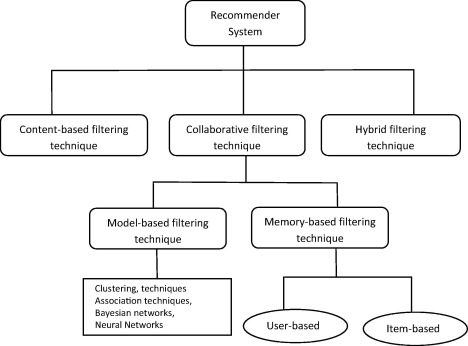
\includegraphics[width=0.7\linewidth]{figures/figure1.jpg}}        
\caption{Recommender systems${^{[1]}}$}
\end{figure}
\hfill

We build a basic content-based recommendation system and collaborative filtering based on user rankings using the MovieLens dataset${^{[2]}}.$ The dataset contains 100,000 ratings on 9,000 movies by 600 users.  ‘movies.csv’ file shows every movie with its id, title, and genre. To describe users' relation with movies we used the ratings.csv file which defines every user with 'userId' and shows their 'rating' based on 'movieId'.
\vspace{4mm}

Firstly we tried to understand the dataset and used some preprocessing steps to get more correct results. Then we build content-based filtering by calculating correlation.  In collaborative filtering, we used two approaches. The first one was turning data into a sparse matrix and getting recommendations based on n-neighbors with the KNN algorithm. In the second one, which is matrix factorization, we used SVD to predict movies for each user based on similarity with users.

\pagebreak

\begin{figure}[h!t]
\centering
{\centering
    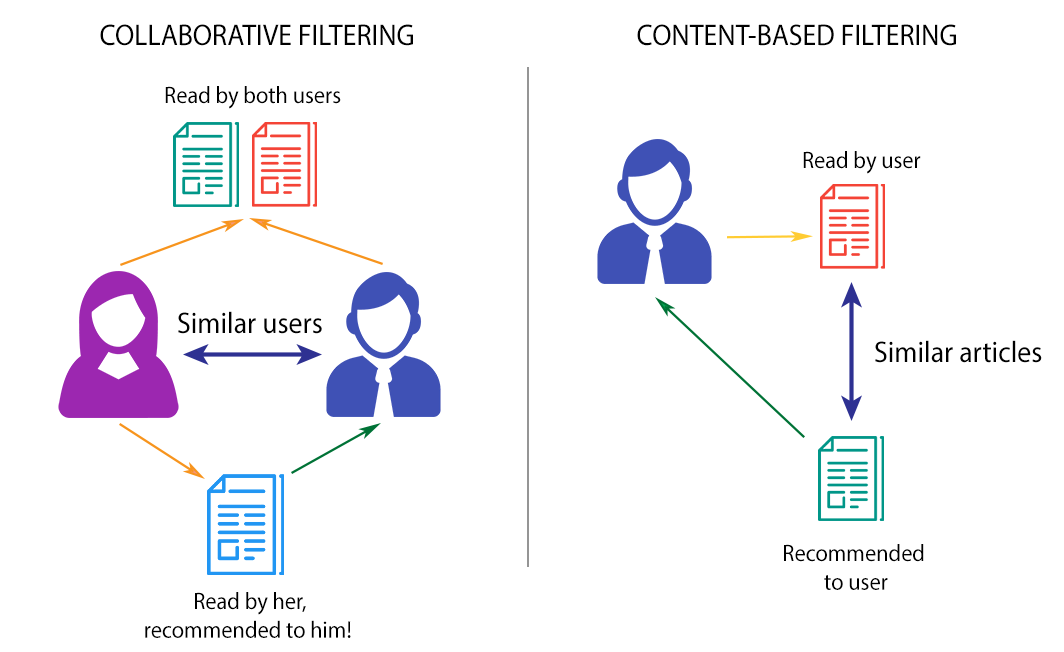
\includegraphics[width=0.7\linewidth]{figures/figure2.png}}        
\caption{Collaborative Filtering \& Content-Based Filtering${^{[4]}}$}
\end{figure}

\hfill

We built a basic GUI, with a small dataset with more attributes which is the IMDB movie dataset${^{[3]}}$. We implemented the GUI with python’s ‘Tkinter’ module.

\begin{figure}[h!t]
\centering
{\centering
    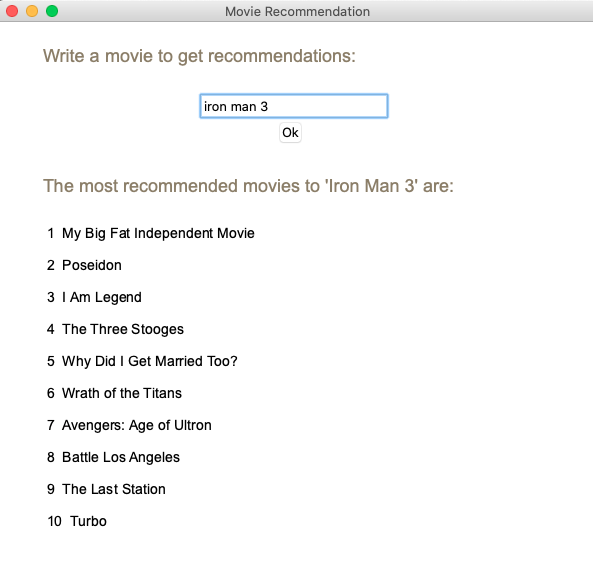
\includegraphics[width=0.7\linewidth]{figures/gui.png}}        
\caption{Our GUI for content-based filtering.}
\end{figure}

\pagebreak

\subsection{Content Based Recommender}
\hspace{0.5cm}This filtering strategy is based on data provided about the items. The algorithm recommends movies similar to the movie the user likes. This similarity is calculated with the cosine similarity of the movie the user likes to all movies in the data set, and the movies with the highest similarity ratio are recommended to the user. For example, if a user likes movies such as ‘The Prestige’ then the system can recommend him the movies of ‘Christian Bale’ or movies with the genre ‘Thriller’ or maybe even movies directed by ‘Christopher Nolan’.So what happens here the recommendation system checks all data of  “The Prestige”, then tries to find similar movies to that using the information available in the database such as the lead actors, the director, genre of the film, production house, etc and based on this information finds movies similar to “The Prestige”. The advantages of the Content-Based approach are that data of other users is not required and the recommender engine can recommend new items that are not rated currently.

\hfill

\begin{figure}[h!t]
\centering
{\centering
    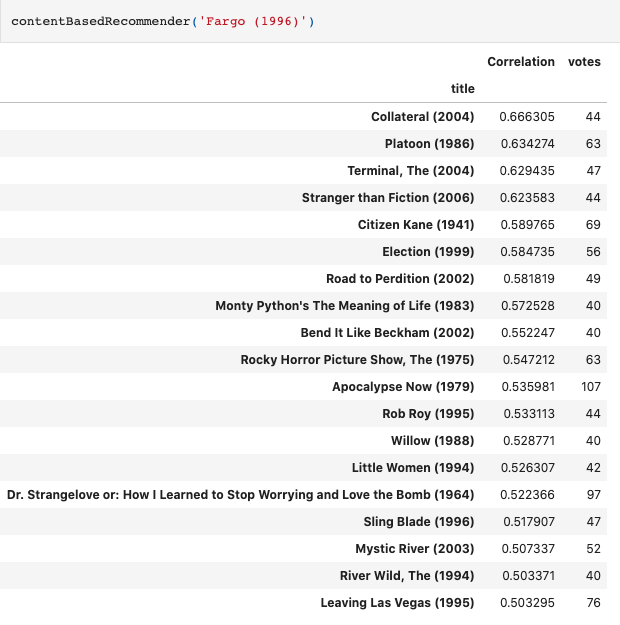
\includegraphics[width=0.8\linewidth]{figures/result1.png}}        
\caption{Content based filtering result for movie 'Fargo'}
\end{figure}



\subsection{Collaborative Filtering}
\hspace{0.5cm}It is based on the idea that people who share the same interest in certain kind of items will also share the same interest in some other kind of items unlike content based which basically rely on metadata while it deals with real-life activity. Collaborative filtering is divided into many methods within itself. We used user-based filtering and matrix factorization in our project.
\hfill

\subsubsection{User-Based Filtering with KNN Algorithm}
\hspace{0.5cm}The basic idea of the collaborative filtering recommendation algorithm is to introduce the information of similar-interest users to object users. User A loves movies A, B, C, and user C likes movies B, D, so we can conclude that the preferences of user A and user C are very similar. Since user A loves movie D as well, so we can infer that user A may also love item D, therefore item D would be recommended to the user.

\vspace{4mm}

The basic idea of the algorithm is based on records of the history score of the user. Find the neighbor user as u` who has the similar interest with target user u, and then recommend the items which the neighbor user u` loved to target user u, the predicted score which targets user u may give on the item is obtained by the score calculation of neighbor user u` on the item. The algorithm consists of three basic steps: user similarity calculation, nearest neighbor selection, and prediction score calculation.

\vspace{4mm}

The similarity between users is calculated by evaluating the value of the items evaluated by two users. The similarity of u and is denoted u' as sim(u,u'), the commonly used method of calculating user similarity is Cosine Similarity. The method calculates the similarity between two users by calculating the cosine of the angle between the two vectors.
After the calculation of similarity as sim(u, u') between users, then the algorithm selects a number of users with the highest similarity as the U’s neighbor denoted as u'. set a fixed value K for the neighbor selection, select only the most K high similarity as neighbors regardless of the value of the neighbor similarity of users. After determining the user's neighbors, the score can be predicted according to the score of the neighbor to the item.


\begin{figure}[h!t]
\centering
{\centering
    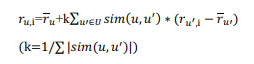
\includegraphics[width=0.4\linewidth]{figures/formula.png}}        
\caption{The calculation formula 
($r_u,i$ as used to predict the score of user u to movie i)}
\end{figure}

\pagebreak

\begin{figure}[h!t]
\centering
{\centering
    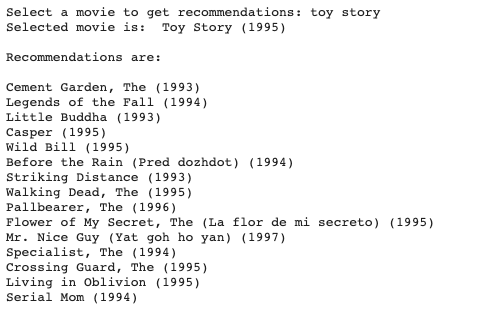
\includegraphics[width=0.8\linewidth]{figures/result2.png}}        
\caption{KNN algorithm result for movie 'Toy Story'}
\end{figure}

\vspace{10mm}

\subsubsection{Matrix Factorization}
\hspace{0.5cm}Matrix factorization comes in limelight after Netflix's competition (2006) when Netflix announced prize money of \$1 million to those who will improve its root mean square performance by 10\%. Netflix provided a training data set of 100,480,507 ratings that 480,189 users gave to 17,770 movies.
\vspace{4mm}

Matrix factorization is the collaborative based filtering method where matrix m*n is decomposed into m*k and k*n. It is basically used for the calculation of complex matrix operations. Division of matrix is such that if we multiply factorized matrix we will get the original matrix.

\pagebreak
\textbf{The Singular Value Decomposition (SVD)}, a method from linear algebra that has been generally used as a dimensionality reduction technique in machine learning. SVD is a matrix factorization technique, which reduces the number of features of a dataset by reducing the space dimension from N-dimension to K-dimension (where K<N). In the context of the recommender system, the SVD is used as a collaborative filtering technique. It uses a matrix structure where each row represents a user, and each column represents an item. The elements of this matrix are the ratings that are given to items by users.

\hfill

\begin{figure}[h!t]
\centering
{\centering
    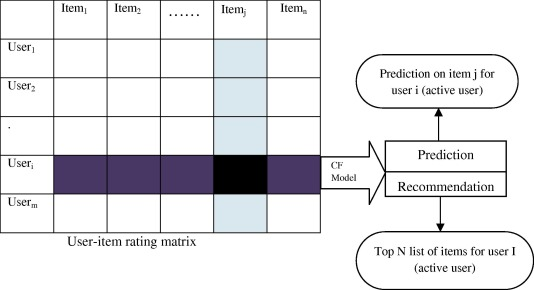
\includegraphics[width=0.8\linewidth]{figures/figure3.jpg}}        
\caption{Collaborative Filtering Process${^{[5]}}$}
\end{figure}

\hfill

\begin{figure}[h!t]
\centering
{\centering
    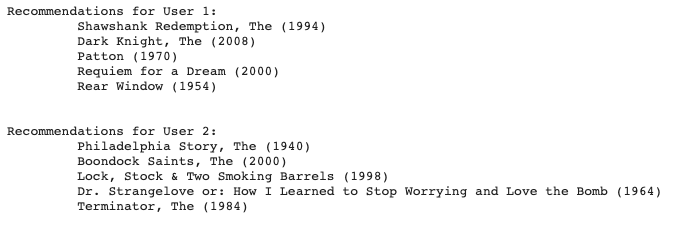
\includegraphics[width=14.1cm]{figures/result3.png}}        
\caption{Matrix Factorization method gives recommendations for each user.}
\end{figure}

\pagebreak

\section{\textbf{Conclusion}}
\vspace{2mm}
\hspace{0.5cm}Machine learning is a method of data analysis that automates analytical model building. It is a branch of artificial intelligence based on the idea that systems can learn from data, identify patterns and make decisions with minimal human intervention.Recommender systems add value to businesses by assisting their customers in selecting the right product out of uncountable choices.In this project , a movie recommender system is built using the content based and collaborative filtering  algorithms. The data are taken from movielens dataset and IMDB movie dataset. The system is implemented in python programming language and also GUI was implemented for IMDB dataset using the python library.



\vspace{20mm}
\Large\textbf{References}\normalsize{}

\rule{140mm}{0.3mm}

\href{https://www.sciencedirect.com/science/article/pii/S1110866515000341}{[1] Figure 1}
\vspace{5mm}

\href{http://files.grouplens.org/datasets/movielens/ml-latest-small.zip}{[2] MovieLens Dataset}
\vspace{5mm}

\href{https://data.world/promptcloud/imdb-data-from-2006-to-2016}{[3] IMDB Movie Dataset}
\vspace{5mm}

\href{https://towardsdatascience.com/brief-on-recommender-systems-b86a1068a4dd}{[4] Figure 2}
\vspace{5mm}

\href{https://ars.els-cdn.com/content/image/1-s2.0-S1110866515000341-gr3.jpg}{[5] Figure 3}
\vspace{5mm}


\nocite{*}
\bibliographystyle{plain}
\bibliography{references}
\end{document}